

If we measure an aspect of security before and after a change takes place, then we can quantify the impact that change had on security. If we test an aspect of cyber security at regular intervals, then we can determine the rate of change for that property over time. In order to sample security measurements at regular (approaching continuous) intervals, we assert that the test apparatus must be fully automated. The necessity of such automation is critical to evaluating security metrics in a repeatable and consistent way. 

% \begin{figure}[ht]
% \centering
% 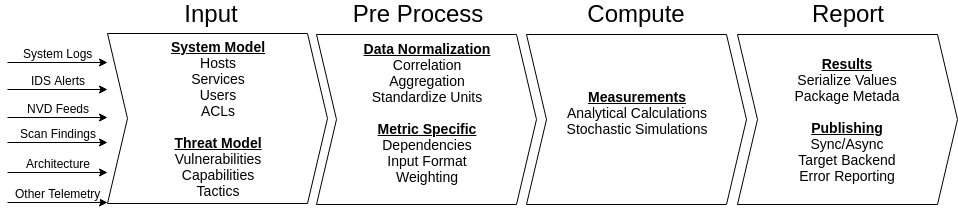
\includegraphics[width=\linewidth]{img/metric_calc_pipeline.png}
% \caption{Generalized Metric Evaluation Pipeline}
% \label{fig:automation:metric_pipeline}
% \end{figure} 

In Figure \ref{fig:automation:metric_pipeline} we present a general four-stage pipeline for security metric processing based on our observations implementing a number of metrics from the literature. This abstraction encourages us to:
\begin{itemize}
\item Decouple the source of system information from the representation of that information. 
\item Decouple the actual calculation of the metric from the input model representation it is typically paired with in its publication. 
\item Decouple the calculation logic and supporting metadata from any assumptions about how that measured value will be used in the future. 
\end{itemize}

In doing so, it becomes possible to identify shared dependencies among metrics, enables a systematic examination of the characteristics and behaviours of each metric across a range of inputs, and supports more reusable and composeable components for a greater variety of deployment scenarios. The remainder of this section provides the considerations and details of each stage.

The number of security metrics available in the literature is somewhat overwhelming. Surveys of security metrics from many\cite{Bohme_Nowey_2008, Haque_Keffeler_Atkison_2017, Hecker_2008, Kordy_2013, Kundu_Ghosh_Chokshi_Ghosh_2012, Pendleton_Garcia-Lebron_Cho_Xu_2016, Ramos_Lazar_Filho_Rodrigues_2017, Rudolph_Schwarz_2012, Savola_2007, Tavallaee_Stakhanova_Ghorbani_2010, Verendel_2009,  Wagner_Eckhoff_2015} sources and perspectives have been conducted, resulting in a multitude of taxonomies for each declaring when and where and how a metric should be applied.  What is notably lacking from these surveys, and indeed from much of the literature reviewed, is any empirical evaluation of the values measured by a given metric. The study of security metrics lacks the context needed to support adoption. What we provide in this chapter is a mechanism to establish the needed context by answering how well do these metrics perform individually across a variety of scenarios, and how do they compare with each other for a given model. To build context for security metrics, we break up our experiments into two parts. 

The first part \textit{sizes} the metric, examining how it behaves across different types and scales of input networks. We apply the metrics implemented in Section \ref{sec:automation:secmet_impl} to a set of models representative of different deployment scenarios. These models include enterprise networks and core networks at scales we label small, medium, and large. The models  act as a reference set against which we can evaluate properties of the implemented metrics. Our primary questions are how do these metrics perform as the size of the system changes, and how do they perform in different types of systems. As our reference set grows, we can develop an understanding of the fundamental or universal security properties we can measure, along with the best metrics for a specific situation. 

The second part \textit{ranges} the metric, examining how it behaves as the security of the system under test changes. We select a system model from our standard set and generate an attack model for a scenario. The range of transition values in the attack model varies by metric, but we can, in the general case, fix these values to present a minimally and maximally secure model with respect to the chosen metric. This bounds the security of a system to a specific range, and measurements within this interval characterize the behaviour of the metric for a scenario. We make observations about monotonicity and sensitivity with respect to a metric and describe properties common across metrics. 

We consider ranging and sizing as two aspects of security metric benchmarking. By benchmarking security metrics we validate their fitness for use in general scenarios, and create reference against which we can measure future security metrics. The rest of this chapter describes the design, testing, and findings from this research. 